\section{Auswertung}
\label{sec:Auswertung}

\subsection{Zeitkonstante eines RC-Kreises} % (fold)
\label{sub:Zeitkonstante}

\noindent Wie in \autoref{sub:Entladekurve_durch} beschrieben, werden $12$ Messwerte aus \autoref{fig:Entladekurve} abgelesen und in \autoref{tab:Entladekurve} dargestellt.
Zudem wird der Logarithmus von dem Verhältnis der Kondensatorspannung $U_C$ zur angelegten Spannung $U_0$ berechnet. $U_0$ beträgt hierbei \qty{1}{\volt},
die Frequenz wird auf \qty{110.7}{\hertz} eingestellt.

\begin{minipage}[t]{0.5\textwidth}
\begin{figure}[H]
  \centering
  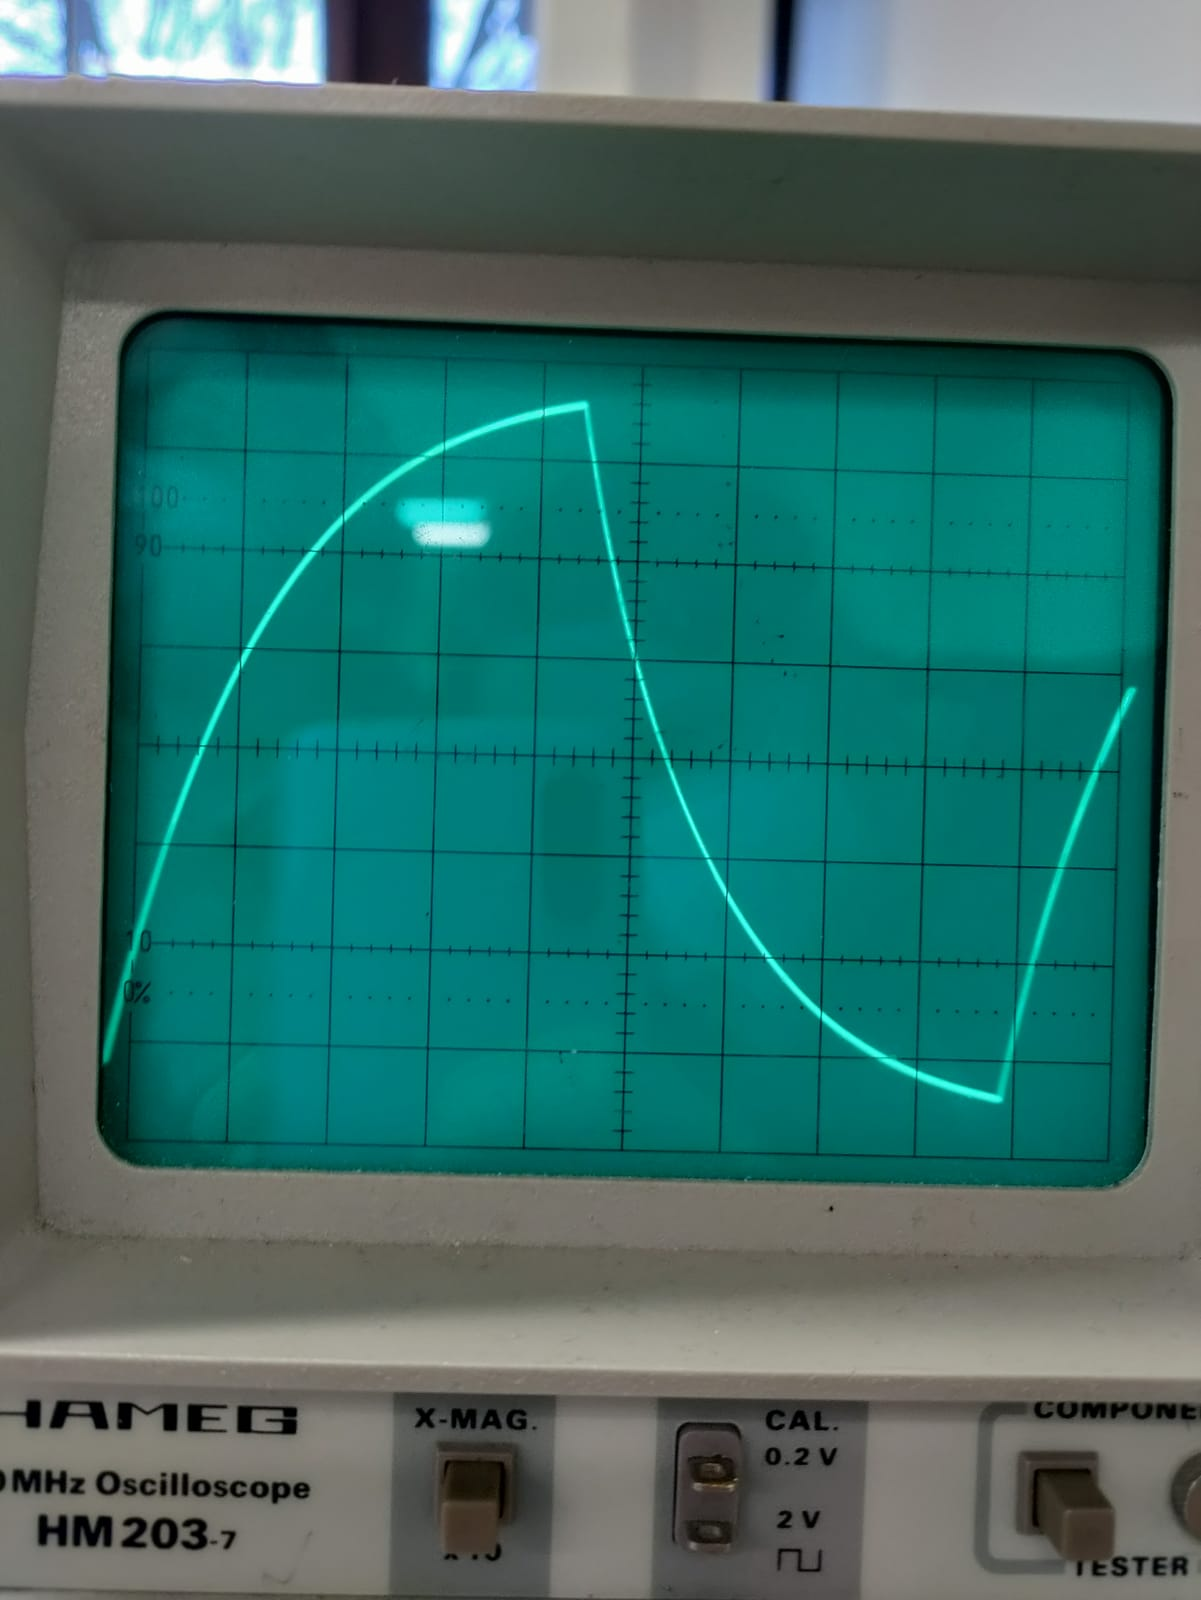
\includegraphics[width=0.69\textwidth]{build/Entladekurve.jpeg}
  \caption{Entladekurve des RC-Kreises\\am Oszilloskop.}
  \label{fig:Entladekurve}
\end{figure}
\end{minipage}
\begin{minipage}[t]{0.5\textwidth}
\begin{table}[H]
  \centering
  \sisetup{table-format=1.1}
  \begin{tabular}{S S[table-format=2.1] S[table-format=3.1]}
    \toprule
    {$t\mathbin{/} \si{\milli\second}$} & {$U_C \mathbin{/} \si{\volt}$} & {$ln\Biggl(\frac{U_C}{U_0}\Biggr)$}\\
    \midrule
    0.0 &  14.0 & 2.6\\ 
    0.4 &  10.4 & 2.3\\
    0.8 &  7.6  & 2.0\\
    1.2 &  5.0  & 1.6\\
    1.6 &  4.0  & 1.4\\
    2.0 &  2.8  & 1.0\\
    2.4 &  1.8  & 0.6\\
    2.8 &  1.1  & 0.1\\
    3.2 &  0.8  & -0.2\\
    3.6 &  0.4  & -0.9\\
    4.0 &  0.3  & -1.2\\
    4.4 &  0.2  & -1.6\\
    \bottomrule
  \end{tabular}
  \caption{Spannungsverlauf der Entladekurve\\des RC-Kreises.}
  \label{tab:Entladekurve}
\end{table}
\end{minipage}

\noindent Mit GLEICHUNG wird 
Hierzu wird mit dem Pythonmodul Matplotlib \cite{matplotlib} der Y-Achsenabschnitt und die Steigung der linearen Regression $y = a \cdot x + b$, 
sowie die zugehörigen Fehler berechnet.\\
\begin{figure}[H]
  \centering
  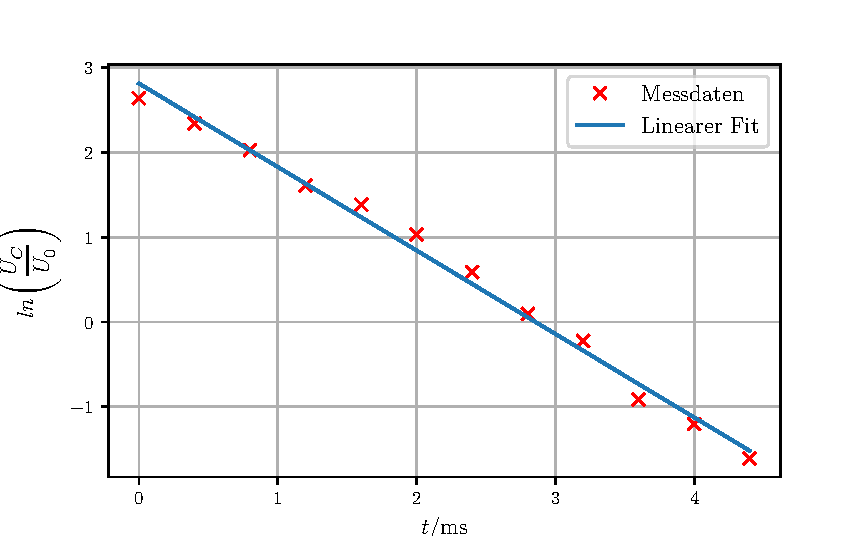
\includegraphics{Entladekurve.pdf}
  \caption{Logarithmierte Kondensatorspannung der Entladekurve gegenüber der Zeit.}
  \label{fig:Entladekurve_plot}
\end{figure}
Mit den Parametern der linearen Regression
\begin{align*}
a &= (-0.99 ± 0.03)\si{\milli\second\tothe{-1}} \\
b &= (2.82 ± 0.07)
\end{align*}
und \autoref{eqn:Zeitkonstante} wird die Zeitkonstante des Relaxationsverhaltens am RC-Kreis zu
\begin{align*}
  RC=(1.02 ± 0.03)\si{\milli\second}
\end{align*}
bestimmt.

% subsection Zeitkonstante  (end)

\subsection{Frequenzabhängige Amplitude und Phasenverschiebung} % (fold)
\label{sub:Freque-A&P}

\begin{table}[H]
  \centering
  \begin{tabular}{
    S[table-format=5.0] 
    S[table-format=1.2] 
    S[table-format=1.1]
    S[table-format=1.4]}
    \toprule
  {$f \mathbin{/} \si{\hertz}$}& {$U_C \mathbin{/} \si{\volt}$} &{$U_0 \mathbin{/} \si{\volt}$} & {$t\mathbin{/} \si{\milli\second}$}\\
    \midrule
    20     & 8.0  & 9.0  & 2.5     \\
    56     & 7.5  & 9.0  & 1.4     \\
    92     & 6.5  & 9.0  & 1.4     \\
    128    & 5.5  & 9.0  & 1.1     \\
    164    & 5.0  & 9.0  & 1.0     \\
    200    & 4.0  & 9.0  & 0.7     \\
    560    & 1.6  & 9.0  & 0.4     \\
    920    & 1.0  & 9.0  & 0.25    \\
    1280   & 0.75 & 9.0  & 0.20    \\
    1640   & 0.6  & 9.0  & 0.15    \\    
    2000   & 0.28 & 9.0  & 0.125   \\
    5600   & 0.17 & 9.0  & 0.04    \\
    9200   & 0.1  & 9.0  & 0.02    \\
    12800  & 0.08 & 9.0  & 0.02    \\
    16400  & 0.06 & 9.0  & 0.015   \\
    20000  & 0.05 & 9.0  & 0.0125  \\
    \bottomrule
  \end{tabular}
  \caption{ganz viel krams}
  \label{tab:Frequenz}
\end{table}

\begin{figure}[H]
  \centering
  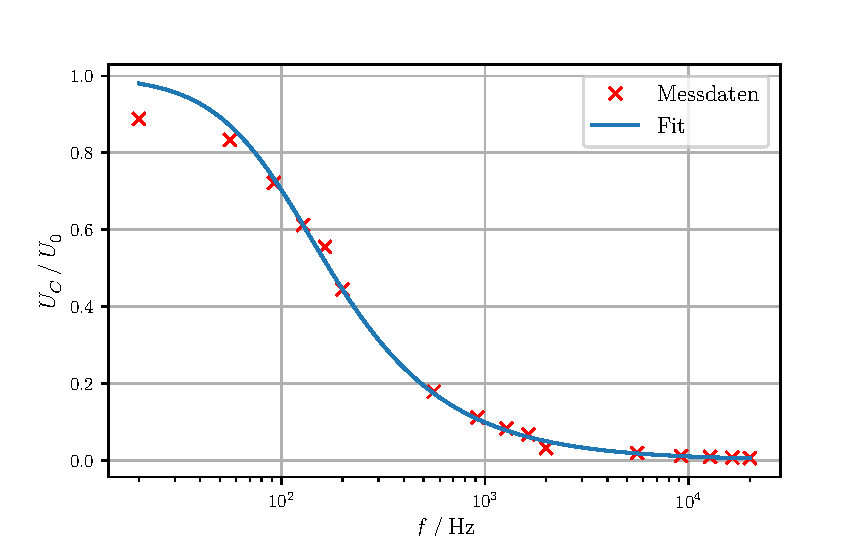
\includegraphics{SpannungFrequenz.pdf}
  \caption{Spannungsverhältnis der Kondensatorspannung zur Generatorspannung gegenüber der Frequenz.}
  \label{fig:SpannungFrequenz_plot}
\end{figure}

\begin{align*}
  RC=(1.61 ± 0.06)\si{\milli\second}
\end{align*}

\begin{figure}[H]
  \centering
  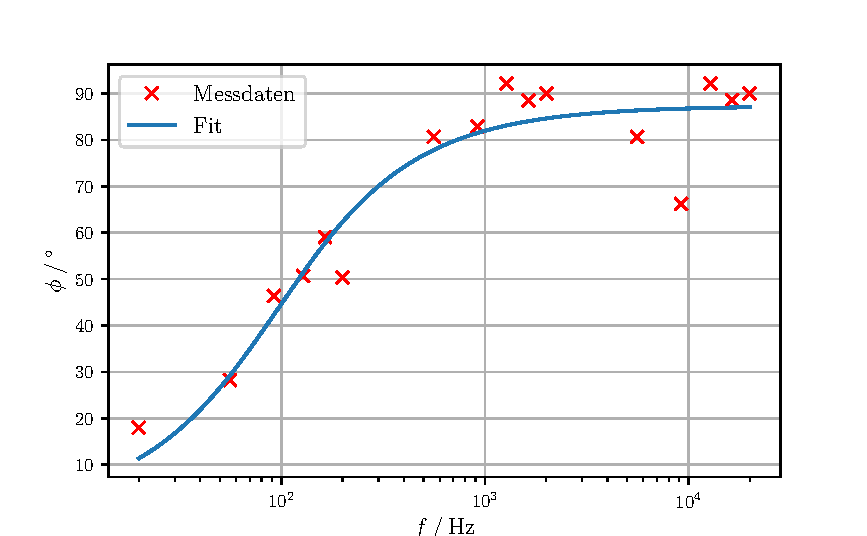
\includegraphics{PhaseFrequenz.pdf}
  \caption{Phasendifferenz der Kondensatorspannung zur Generatorspannung gegenüber der Frequenz.}
  \label{fig:PhaseFrequenz_plot}
\end{figure}
\begin{align*}
  RC=(1.65 ± 0.25)\si{\milli\second}
\end{align*}
Keine Ahnung warum unsere werte so hässlich sind, vielleicht hätten wir das doch genauer ablesen sollen... Naja egal 
 %subsection Frequenzabhängige Amplitude und Phasenverschiebung (end)

\subsection{Ein RC-Kreis als Integrator} % (fold)
\label{sub:Integrator}

% subsection Ein RC-Kreis eines Integrators (end)



Siehe \autoref{fig:plot}!
